Old figure for Rust to SPARK

\begin{figure}[ht!]    \centering
    \begin{tikzpicture}[node distance=2cm, font=\small]
    \tikzstyle{process} = [draw, rectangle, minimum width=5cm, minimum height=1cm, text centered, text width=4.5cm, fill=white, rounded corners=10,thick]
    \tikzstyle{arrow} = [->, >=stealth, thick]
    \node (step1) [process, fill=red!20] {cargo project: main.rs + build.rs \\
        \begin{tikzpicture}[font=\small, scale=0.2, inner sep=2pt]
            \node (lib.adb) [process] {lib.adb};
        \end{tikzpicture}
    };
    \node (step2) [process, fill=yellow!20, below of=step1] {Compiled SPARK library};
    \node (step3) [process, fill=brown!20, below of=step2] {Building};
    
    \draw [arrow] (step1) -- (step2) node[midway, right] {build.rs calls gprbuild};
    \draw [arrow] (step2) -- (step3) node[midway, right] {rustc link};
    \draw [arrow] (step3.south) -- +(0,-0.5) -- +(5.5,-0.5)  node[right] {executable};
\end{tikzpicture}
    \caption{Rust using a SPARK library}
    \label{fig:rustbuild}
\end{figure}


\begin{figure}[!ht]
  \begin{center}
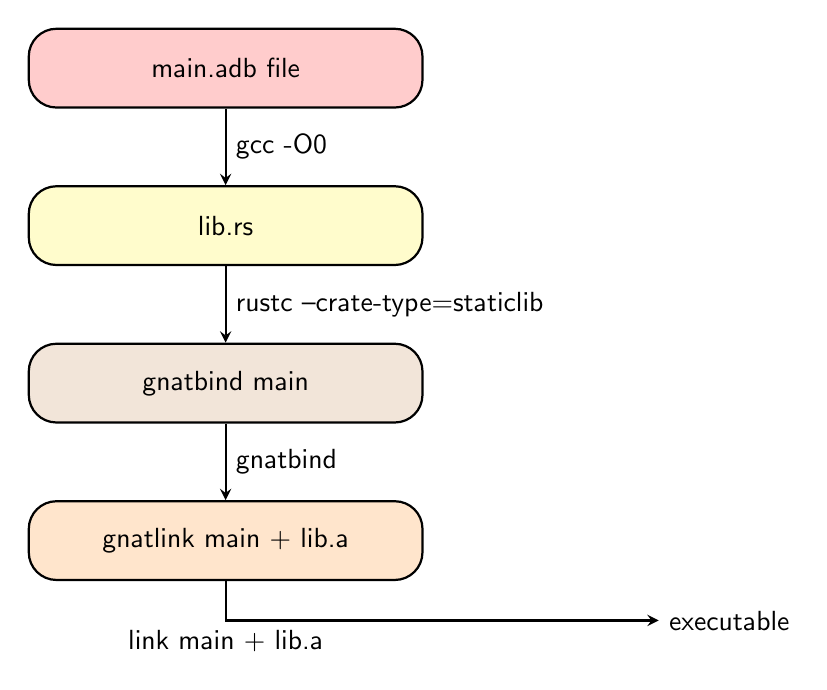
\begin{tikzpicture}[node distance=2cm, font=\sffamily]
    \tikzstyle{process} = [draw, rectangle, minimum width=5cm, minimum height=1cm, text centered, text width=4.5cm, fill=white, rounded corners=10,thick]
    \tikzstyle{arrow} = [->, >=stealth, thick]
    \node (step1) [process, fill=red!20] {main.adb file};
    \node (step2) [process, fill=yellow!20, below of=step1] {lib.rs};
    \node (step3) [process, fill=brown!20, below of=step2] {gnatbind main};
    \node (step4) [process, fill=orange!20, below of=step3] {gnatlink main + lib.a};

    \draw [arrow] (step1) -- (step2) node[midway, right] {gcc -O0};
    \draw [arrow] (step2) -- (step3) node[midway, right] {rustc --crate-type=staticlib};
    \draw [arrow] (step3) -- (step4)
    node[midway, right] {gnatbind};
    \draw [arrow] (step4.south) -- +(0,-0.5) node[below] {link main + lib.a} -- +(5.5,-0.5)  node[right] {executable};
\end{tikzpicture}
  \end{center}
  \caption{SPARK using a Rust library}
  \label{fig:buildada}
\end{figure}


(FFI-checker had dependencies issues, rr had issues on AMD and memflow is designed to track memory down to the operative system, while we were mostly looking at address consistencies)